\clearpage
\title{Problem 7.2}
\author{}
\date{}
\maketitle

\section*{Problem Description}
Sort an array.

\section*{Process}
\subsection*{Code:}

\begin{multicols}{2}{|}
    \begin{minted}[linenos,breaklines,breakanywhere]{nasm}
DATA SEGMENT
    ARR DB 7, 2, 8, 1, 0, 4, 5, 9, 6
DATA ENDS

CODE SEGMENT
    ASSUME DS:DATA, CS:CODE

START:
    MOV AX, DATA
    MOV DS, AX
    
    MOV BX, 8
    XOR AX, AX
    
    LEA SI, ARR
    MOV DX, SI
    
SORT_:
    MOV SI, DX
    MOV CX, BX
    MOV DI, SI
    MOV AL, [DI] 
    
BIG_:
    INC SI
    CMP [SI], AL
    JNG NEXT
    MOV DI, SI
    MOV AL, [DI]
    
NEXT:
    LOOP BIG_
    
    MOV AL, [SI]
    XCHG AL, [DI]
    MOV [SI], AL
    
    DEC BX
    JNZ SORT_
    
CODE ENDS
END START
\end{minted}
\end{multicols}

\subsection*{Output}
\begin{center}
    \centering
    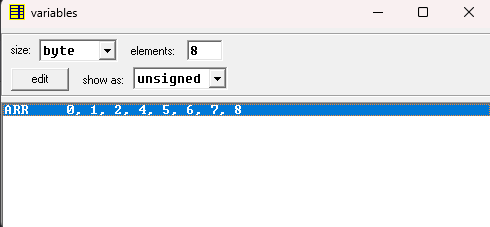
\includegraphics[width = \textwidth]{sort.png}
    \captionof{figure}{Sorted array.}
\end{center}


